\documentclass[11pt, a4paper]{article}

\usepackage[a4paper, top=2.5cm, bottom=2.5cm, left=2cm, right=2cm]{geometry}
\usepackage[utf8]{inputenc}
\usepackage[T1]{fontenc}
\usepackage[english]{babel}

\usepackage{titlesec}
\titlespacing*{\section}{0pt}{1.5\baselineskip}{1\baselineskip}
\titlespacing*{\subsection}{0pt}{1.0\baselineskip}{0.5\baselineskip}

\title{Design Report }
\author{ AFS-Like Distributed File System}
\date{}

\usepackage[hidelinks]{hyperref}
\usepackage{textcomp}
\usepackage{graphicx} % <<< ADDED THIS PACKAGE

\begin{document}

\maketitle
\thispagestyle{empty}
\pagestyle{headings}


\section{Executive Summary}

This report presents the design and implementation of a fault-tolerant AFS Distributed File System for finding prime numbers in large datasets. The system uses a three-tier architecture in which coordinators and file servers are replicated, applies the Raft consensus algorithm for election of new leader file server, employs global snapshots for consistent state capture and crash recovery, and provides fault tolerance through multiple redundancy layers.

System Scale: Multiple Workers, Replicated Coordinators (active-passive), and Replicated File Servers (leader-followers).

Communication: gRPC protocol

Key Algorithms: Global snapshots, Raft consensus, exponential backoff with failover

\section{Failure Types Handled}

Failure Type		Detection				        Recovery									    Guarantee
Client Crash		Alive lock file on restart	    Global snapshot download + task resumption	    Eventually consistent
Coordinator Crash	gRPC timeout		            Failover to secondary coordinator			    High availability
FileServer Crash	gRPC timeout				    Raft leader election						    Linearizable consistency
Network Partition	gRPC deadline exceeded	        Exponential backoff + retry					    Eventually consistent
Data Corruption		Checksum mismatch		        Reject + retry download						    Strong integrity
Task Failure		Client loses heartbeart	        Coordinator times out and reassigns task		At-least-once semantics

\section{Assumptions}

Network Assumptions:
Eventual Connectivity:  Network partitions are transient
Non-Byzantine:          No malicious actors (crash-fail model)
Bounded Latency:        Sufficient gRPC timeouts (30-60 seconds)

Timing Assumptions:
Partially Synchronous:  Bounded message delays

Storage Assumptions:
Persistent Storage:     File servers have durable storage
Atomic Rename:          POSIX-compliant file systems
No Silent Corruption:   Disk errors

Process Assumptions:
Fail-Stop:              Processes crash cleanly (no stuck states)
Independent Failures:   Worker crashes are uncorrelated

\section{Limitations Not Handled}
Byzantine Failures:                 Malicious clients/servers
Network Delays > Timeout:           Premature timeouts treated as failures
Concurrent Coordinator Failures:    Requires manual intervention
File Server Quorum Loss:            System halts if > N/2 servers fail
Disk Corruption:                    Silent data corruption not detected beyond checksums

\section{System Model}

This report explains the design for a distributed fault tolerant system that finds unique prime numbers and store them in a file server.

\begin{itemize}
    \item \textbf{System Model:} The system is consists of the following (File Servers, Coordinator, Workers) communicating over an asynchronous network. Processes and network links can fail (e.g., crash failures, network partitions).

    \item \textbf{Core Components:}
          \begin{enumerate}
              \item \textbf{File Primary and Replicated Servers:} A replicated, high-availability file server based on the Raft consensus algorithm.
              \item \textbf{Application Coordinators:} A central service that manages the task assignments, splits work, and triggers snapshots.
              \item \textbf{Application Workers:} A Worker process that requests tasks from the Coordinator, performs computation, and interacts with the File Servers.
          \end{enumerate}
\end{itemize}


\section{AFS Distributed File System}

The file system provides highly-available storage for input datasets and output results as shown in Figure (1).

\begin{figure}[htbp]
    \centering
    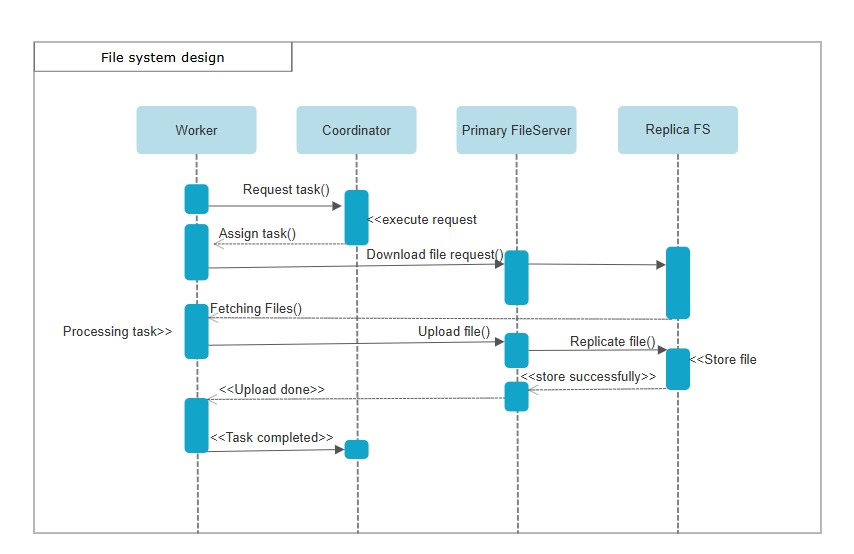
\includegraphics[width=0.9\textwidth]{system-design.jpeg}
    \caption{File system design sequence diagram.}
    \label{fig:system_design}
\end{figure}

\subsection{Architecture \& Core RPCs}

The system communications falls under the following RPC commands:


\begin{itemize}
    \item UploadFile(stream FileChunk): Handles worker file uploads (writes).
    \item FetchFile(FetchRequest): Handles worker file downloads (reads).
    \item RequestVote(VoteRequest): Internal Raft RPC for leader election.
    \item Heartbeat(HeartbeatRequest): Internal Raft RPC for leader authority and liveness.
    \item ReplicateFile(stream ReplicateFileRequest): Internal RPC for the leader to push file data to followers.
\end{itemize}



\newpage
\subsection{Fault Tolerance}

High availability is achieved at multiple levels. For the application, a backup coordinator and task re-assignment logic are used. For the file servers, the \textbf{Raft consensus algorithm} is used, not a simple primary-backup.


\subsubsection*{Application Fault Tolerance}
\begin{itemize}
    \item \textbf{Coordinator Failure (Backup Coordinator):} To prevent the Coordinator from being
          a single point of failure, a backup Coordinator runs in the background.
          If the primary Coordinator fails (detected via missed heartbeats), the backup takes over.
          Workers are configured to automatically connect to the backup's address.

    \item \textbf{Worker Failure (Heartbeating):} Workers send periodic heartbeats to the Coordinator.
          If the Coordinator does not receive a heartbeat from a worker after a set timeout,
          it marks the worker as 'dead' and the task as 'failed' and assigns it to another worker.

    \item \textbf{Task Re-assignment \& Snapshots:} When a task is marked as failed,
          the Coordinator re-assigns it to a new, available worker.
          To avoid starting from scratch, workers periodically save their progress
          to the file system. The new worker loads this snapshot and resumes computation
          from the last checkpoint.
\end{itemize}

\newpage

\subsubsection*{File Server Fault Tolerance (Raft)}


\begin{itemize}
    \item \textbf{Leader Election:} Servers start as (Follower). If no heartbeats are received from a leader within a randomized timeout, a server becomes a (Candidate), increments its term, and requests votes. If it wins a majority, it becomes (Leader).
    \item \textbf{Write Path (Leader-Only):} All write operations (UploadFile) are handled exclusively by the leader. If a worker contacts a follower, the follower rejects the request, and the worker is responsible for retrying with another server until it finds the leader.
    \item \textbf{Replication Path:}
          \begin{enumerate}
              \item The Leader accepts an (UploadFile) stream from a worker.
              \item It commits the file to its local storage and updates its in-memory file map (version, checksum, etc.).
              \item It then triggers an asynchronous replication to all followers.
              \item The Primary server calls the ReplicateFile RPC on each follower, streaming the new file data to them.
          \end{enumerate}
    \item \textbf{Read Path (Read-Optimized):} Any server (Leader or Follower) can service a FetchFile request. This aligns with the read-heavy AFS-like specification, allowing read load to be balanced across all nodes.
\end{itemize}


\end{document}